\chapter{Method}\label{ch:method}
\section{Main idea}\label{sec:main idea}
In this chapter, the algorithm, how to use homography transformation to do image registration is introduced. It will start with the camera projection to get 3D projection transformation. Then it is simplified to 2D projection with the constrains of points on a plane i.e. Homography transformation. Finally,  the algorithm of multiple homography will be introduced. 
\subsection{Projection of Points on a Plane}
Camera projection is a projection progress for a set of points from world coordinate system to image coordinate system, i.e. to calculate a projection matrix between these two coordinate system, which is called camera matrix $P$. And the exact definitions of different coordinates is in \cref{def: world coordinate system}, \cref{def: camera coordinate system}, \cref{def: image coordinate system} and \cref{def: pixel coordinate system}.

\begin{figure}[htbp]
	\centering
	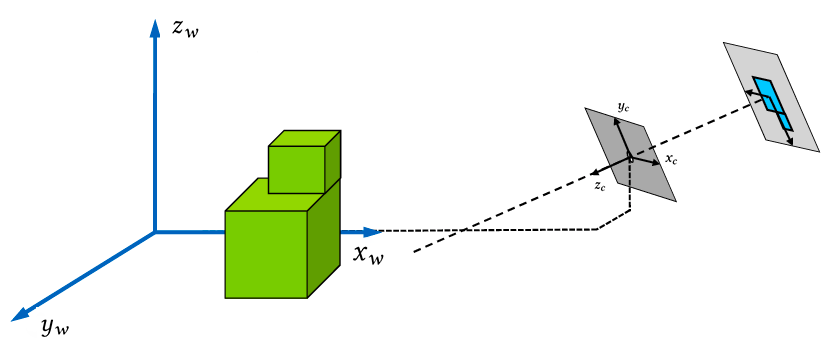
\includegraphics[width=0.80\textwidth]{images/World_to_camera}
	\caption{World to image mapping \cite{collinsPlanarHomographies}}
	\label{fig:worldtocamera}
\end{figure}

Just like \ref{fig:worldtocamera} shows, the first step is to transform from world coordinate to camera coordinate. The extrinsic parameter is the 3 by 3 rotation matrix $R$ of camera coordinate system relative to the world coordinate system and the location $\rdc$ of the camera center in the world coordinate system. The mapping is describe as: (in the equation, $\vec{0}_{3}$ means a vector of three zeros.)
\begin{align}\label{eq:world to camera}
	\begin{pmatrix}
	 		x_c\\
	 		y_c\\
	 		z_c\\
	 		1
	\end{pmatrix}=
	\begin{bmatrix}R^T & -R^T \rdc \\
		\vec{0}_{3}^T & 1
	\end{bmatrix}
	 \cdot \begin{pmatrix}
	x_w\\y_w\\z_w\\1
\end{pmatrix}
\end{align}
Then with the 3 by 3 calibration matrix $K$ (consists of intrinsic parameters), the coordinate is transformed to pixel coordinate as 
\begin{align}\label{eq:camera to pixel}
	\begin{pmatrix}
		u\\
		v\\
		1
	\end{pmatrix} \propto z_c \begin{pmatrix}
	u\\
	v\\
	1
	\end{pmatrix} = \begin{bmatrix}
	K&\vec{0}_{3}\end{bmatrix} \cdot \begin{pmatrix}
	x_c\\
	y_c\\
	z_c\\
	1
\end{pmatrix}
\end{align}
Combine \cref{eq:world to camera} and \cref{eq:camera to pixel}, 
\begin{align}
\begin{pmatrix}
u\\
v\\
1
\end{pmatrix} \propto z_c\begin{pmatrix}
u\\
v\\
1
\end{pmatrix} = \begin{bmatrix}
K&\vec{0}\end{bmatrix} \cdot \begin{bmatrix}R^T & -R^T \rdc \\
\vec{0}^T & 1 \end{bmatrix} \cdot \begin{pmatrix}
x_w\\y_w\\z_w\\1
\end{pmatrix}
\end{align}
And the middle part is the 3 by 4 camera matrix $P$, which describes the mapping of a pinhole camera from 3D points in the world to 2D points in an image.
\begin{align}
P= KR^T \begin{bmatrix}I_{3} & -\rdc \end{bmatrix}
\end{align}
Here distortion is ignored to ensure that it is a linear transformation.

When the object more specifically the points of object $\rdx$is on one plane and $\vec{n}$ is defined as the unit outward normal vector of plane, then the scalar product $\rdx \cdot \vec{n}$ is constant. Thus the camera matrix will be simplified to a 3 by 3 matrix, called homography matrix $H$. Suppose the plane is on the x-y plane in the world, detailed process of this shows in the \cref{fig:planar projection}. The homography matrix between world and image coordinate is finally simplified to:
\begin{align}
H = \begin{bmatrix}
h_{11} &h_{12} & h_{13}\\
h_{21} &h_{22} &h_{23}\\
h_{31}&h_{32}&h_{33}
\end{bmatrix}
\end{align}
\begin{figure}[htbp]
	\centering
	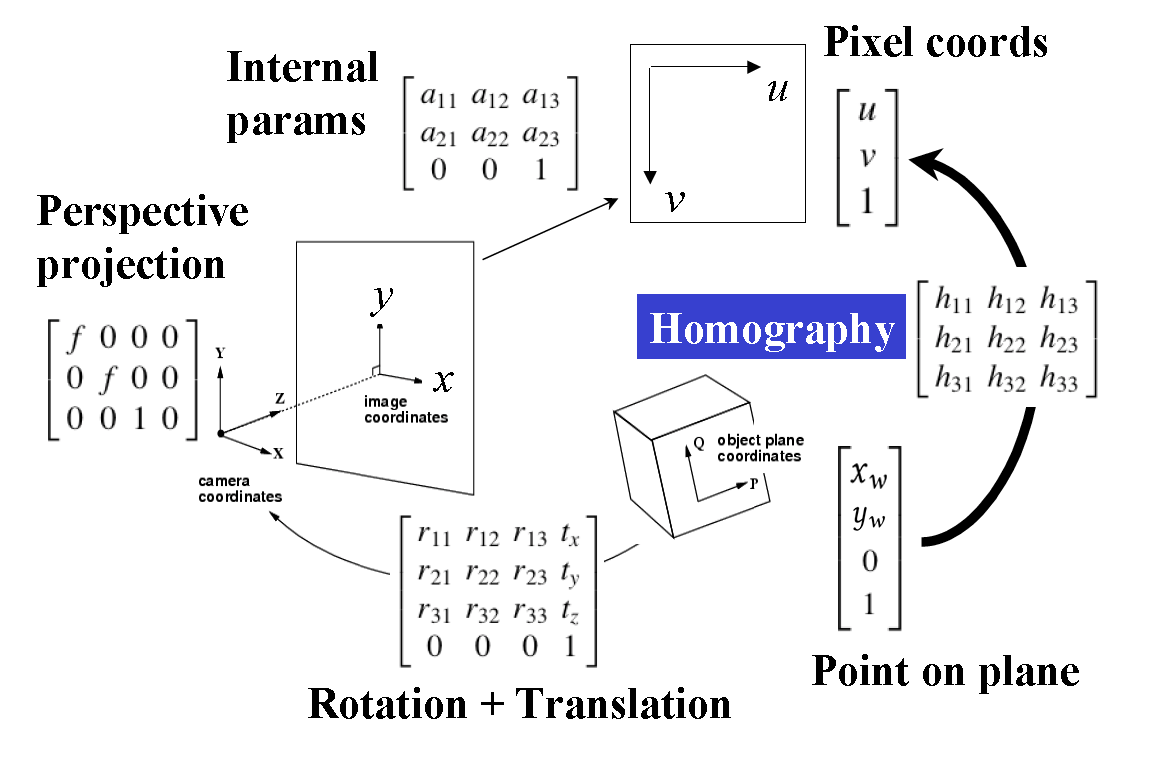
\includegraphics[width=0.80\textwidth]{./images/Planar Projection.png}
	\caption{Planar projection \cite{collinsPlanarHomographies}}
	\label{fig:planar projection}
\end{figure}
Go further, when there is a planar object in two different cameras or one camera with different poses, we can get two homography matrix $ H_{1}$ and $H_{2}$ for this two transformation. Then the homography matrix $H_{2\leftarrow1}$ between this two images of the same object can be calculate as:
\begin{align} 
H_{2\leftarrow1} = H_{2}\cdot H_{1}^{-1}
\end{align}
We assume that two fixed uncalibrated cameras give rise to two camera matrices $P_{1} = K_1R_1^T[I_3, -\rdc_{1}]$ and $P_{2} = K_{2}R_{2}^T[I_{3}, -\rdc_{2}]$. Moreover, these two cameras photograph the same plane $n$ with a unit outward normal $\vec{n}_{n}$ situated at a distance $d_{n}$ from center $\rdc_{1}$ of camera 1. Then the plane $n$ gives rise to a planar homography from the camera 1 to camera 2: \cite{chojnackiEnforcingConsistencyConstraints2015} \cite{bakerParameterizingHomographies}
\begin{align}\label{eq:homography}
H=K_{2}R_{2}^T(I-\frac{(\rdc_{2}-\rdc_{1})\vec{n}_n^{T}}{d_n})R_{1}K_{1}^{-1}
\end{align}
where  
\begin{itemize}
	\item $\rdc_{1},\rdc_{2}$ : location of the camera center in the world coordinate system
	\item $R_{1},R_{2}$: rotation matrix of camera coordinate system relative to the world
	\item $K_{1},K_{2}$: calibration matrix of camera
	\item $\vec{n}_n$: unit outward normal vector of plane
	\item $d_n$: distance from the plane to camera center $\rdc$ and $d_n = \vec{n}_n\left(\rdx - \rdc_{1}\right)$ for any point $\rdx$ on the plane
\end{itemize}

\begin{definition}[World coordinate system]\label{def: world coordinate system}
	World coordinate system $(x_w, y_w, z_w, 1)^T$is the right handed cartesian coordinate system where people take the picture . The unit is meter.
\end{definition}
\begin{definition}[Camera coordinate system]\label{def: camera coordinate system}
	Camera coordinate system $(x_c, y_c, z_c, 1)^T $ is established on the camera in order to describe the position of object from perspective of camera, as a middle link between the world coordinate system and the image/pixel coordinate system. In the thesis,  the origin is set at the center of camera in meters, $z$ axis is pointing from the center of camera to object, $y$ axis is upwards and $z$ axis points to right.
\end{definition}
\begin{definition}[Image coordinate system]\label{def: image coordinate system}
	Image coordinate system$(x, y, 1)^T$ is established on the image in order to describe how locations are measured in the image and the projection transmission relationship of the object from camera coordinate to pixel coordinate during camera projection. In the thesis, the origin is set at the center of image in meters.
\end{definition}
\begin{definition}[Pixel coordinate system]\label{def: pixel coordinate system}
	Pixel coordinate $(u, v, 1)^T$ defines the pixel location as an array in multi-dimensional space. Each image axis has a length, in pixels, so that the image coordinate run between 1 and the length of axis. The total number of pixels in the image equals the product of the axis length for all image axes. In the thesis, the origin is set at the center of the first upper left pixel in the image.
\end{definition}
And in all definitions above have used the homogeneous coordinate in projective geometry. They have the advantage that the coordinates of points, including points at infinity, can be represented using finite coordinates.
\subsection{Multiple Homography} \label{subsec: Multiple Homography calculation}
Just like in \cref{sec: Multiple Homography} introduced, when there are more than one flat planes in the image, only one homography matrix can not describe all the planes. For this situation, the multiple homography is needed. Multiplying out \cref{eq:homography} and rearranging it leads to  
\begin{align} \label{eq:Multiplehomographymatri}
	H=K_{2}R_{2}^T R_{1}K_{1}^{-1}+K_{2}R_{2}^T(\rdc_{1}-\rdc_{2})\cdot \frac{\vec{n}_n^{T}}{d_n}R_{1}K_{1}^{-1}
\end{align}
and define that,
\begin{itemize}
	\item $H_{\infty}=K_{2}R_{2}^T R_{1}K_{1}^{-1}$
	\item $\vec{e}=K_{2}R_{2}^T(\rdc_{1}-\rdc_{2})$
	\item $\vec{q}_{n}^T=\frac{\vec{n}_n^{T}}{d_n}R_{1}K_{1}^{-1}$
\end{itemize}
Among them, $H_{\infty}$ represent the homography matrix for the plane at infinity, $\vec{e}$ is the epipole in the second view, and $\vec{q}_n$ means a $3 \times 1$ vector for the plane $n$, which all the points belongs to. Finally, the homography matrix for plane $n$ is
\begin{align}\label{eq:homography_infty}
	H_{n} = H_{\infty} + \vec{e} \cdot \vec{q}_{n}^T
\end{align}

If the homography $H_{\infty}$ at infinity can't be found,  a homography matrix $H_{0}$ for an exist plane can be used as reference plane and all other planes can be expressed in terms of $H_0$ with:
\begin{align}\label{eq:homography_0}
H_{0} = H_{\infty} + \vec{e} \cdot \vec{q}_{0}^T
\end{align}
And for another plane $n$ in the same image, $\vec{p}_{n}^T$ is defined as $\vec{p}_{n}^T = \vec{q}_{n}^T -\vec{q}_{0}^T$. With \cref{eq:homography_0}, the new form of homography matrix for plane $n$ is got
\begin{align}\label{eq:homography_i}
	H_{n} = H_{0} + \vec{e} \cdot \vec{p}_{n}^T
\end{align}
In this equation, $H_{0}$ is a global and constant value for the whole image, $\vec{e}$ is also a global variable (the epipole in the second view) for the whole image. And $\vec{p}_{n}^T$ is different for different planes. Therefore,  \cref{eq:homography_i} is an express of multiple homography with two global variables $H_{0}$, $\vec{e}$ and one local variable $\vec{p}_{n}^T$. People can use it to transform the plane in one image to another or build the corresponding matching for the same plane in different images.  The algorithm also use this multiple homography to transform the plane and make image registration per plane.
